\chapter{Convex sets and functions}
\label{chap:convex_sets_functions}

\section{Convex sets}  
\label{sec:convex_sets}

Convex sets serve as key building blocks for the study of convex functions and
convex optimization, as essentially everything that can be said about the
latter can be traced back to a statement about convex sets. A set $C \subseteq
\R^d$ is called \emph{convex} if it satisfies   
\index{convex set} 
\begin{equation}
\label{eq:convex_set}
x, y \in C \implies t x + (1-t) y \in C, \quad \text{for all $t \in [0,1]$}. 
\end{equation}
This condition says that the line segment $\{ tx + (1-t) y : t \in [0,1] \}$
joining $x$ and $y$ lies entirely in $C$. See Figure \ref{fig:convex_set}. A
\emph{convex combination} of points $x_1,\ldots,x_n \in \R^d$ is one of the form    
\index{convex combination} 
\[
\sum_{i=1}^n t_i x_i, \quad \text{where $t_i \geq 0$, for $i=1,\ldots,n$ and 
  $\sum_{i=1}^n t_i = 1$}. 
\] 
The \emph{convex hull} of $C$ is the set of all convex combinations of points in
$C$, 
\index{convex hull} 
\[ 
\conv(C) = \bigg\{
\sum_{i=1}^n t_i x_i : 
\text{$n \geq 1$, $x_i \in C$, $t_i \geq 0$, for $i=1,\ldots,n$, and 
  $\sum_{i=1}^n t_i = 1$} \bigg\}. 
\]
The convex hull $\conv(C)$ is itself a convex set, for any set $C$; in fact, it
is the smallest convex set containing $C$, meaning $\conv(C) \subseteq D$ for 
any convex set $D \supseteq C$. 

\begin{figure}[tb]
\centering
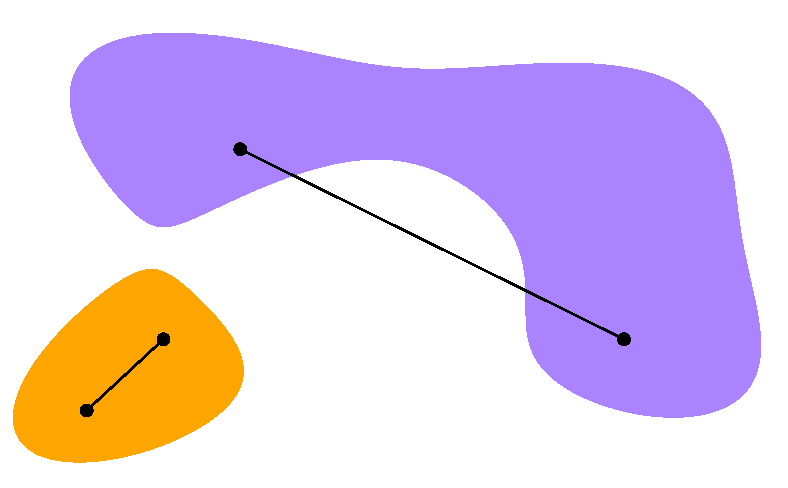
\includegraphics[width=0.65\textwidth]{fig/convex_set.pdf}
\caption{Lower left: convex set, such that the line segment joining any two 
  elements will lie entirely in the set. Upper right: nonconvex set, such
  that this does not hold.} 
\label{fig:convex_set}
\end{figure}

\begin{Example}
The following are examples of convex sets. 

\begin{enumerate}[label=\alph*.]
\item The empty set $\emptyset$, and all of Euclidean space $\R^d$. 

\item A line $\{x + t y : t \in \R\}$, ray $\{x + t y : t \geq 0\}$, and line  
  segment $\{x + t y : t \in [0,1]\}$.

\item A linear subspace $\{x : Ax = 0\}$, and affine subspace $\{x : Ax = b\}$. 

\item A hyperplane $\{x : a^\T x = b\}$, and halfspace $\{x : a^\T x \leq b\}$. 

\item A \emph{norm ball} $\{x : \|x\| \leq t\}$, where $\|\cdot\|$ is a norm on
  $\R^d$, and $t \geq 0$. 
  \index{norm!ball}
  
\item A \emph{polyhedron} $\{x: a_i^\T x \leq b_i, \, i=1,\ldots,m\}$. This is
  the intersection of a finite number of halfspaces. We can express this
  succinctly as $\{x : Ax \leq b\}$, where here and throughout we read the
  inequality componentwise.   
\end{enumerate}
\end{Example}  

It will be important to think about convexity for sets of matrices (and
convexity for functions of matrices), since several optimization problems of
interest are formulated over matrices. By viewing $\R^{k \times d}$---the space   
of real $k \times d$ matrices---as a vector space of dimension $kd$, everything   
we cover for convex sets in $\R^d$ (and convex functions on $\R^d$) can be
translated over to $\R^{k \times d}$. 

The same can be said about $\SS^d$---the space of symmetric real $d \times d$
matrices---which we can view as a vector space of dimension $d(d+1)/2$. A subset
of $\SS^d$ of particular interest is 
\index{positive semidefinite cone} 
\index{positive semidefinite matrix} 
\begin{equation}
\label{eq:psd_cone}
\SS_+^d = \{X \in \SS^d : X \succeq 0 \}.
\end{equation}
Here we write $X \succeq 0$ to denote that $X$ is \emph{positive semidefinite}:
it satisfies $a^\T X a \geq 0$, for all $a \in \R^d$. We call $\SS_+^d$ the
\emph{positive semidefinite cone} (of dimension $d$). This is a convex set,
indeed a \emph{convex cone} which means it satisfies $X,Y \in \SS^d \implies s
X + t Y \in \SS^d$ for all $s,t \geq 0$. To see this, note that for any $s, t
\geq 0$ and $a \in \R^d$, we have  
\[
a^\T (s X + t Y) a = s a^\T X a + t a^\T Y a \geq 0,
\] 
provided that $X,Y$ are positive semidefinite to begin with. 

Given a set $C$ and a point $x \in C$, another interesting convex cone is the
\emph{normal cone} to $C$ at $x$,   
\begin{equation}
\label{eq:normal_cone}
\cN_C(x) = \{ g : g^\T x \geq g^\T y, \, \text{for all $y \in C$}\}.
\end{equation}
For any set $C$ (convex or not), the associated normal cone $\cN_C(x)$ at 
any $x \in C$ is always a convex cone (which can be verified from the
definition). 
\index{normal cone} 

We finish this short section with two key theorems on properties of convex sets. 

\index{separating hyperplane theorem}
\begin{Theorem}[Separating hyperplane theorem]
\label{thm:separating_hyperplane}
If $C,D$ are nonempty disjoint convex sets, then there exists $a \not= 0$ and
$b$ such that $C \subseteq \{x : a^\T x \leq b\}$ and $D \subseteq \{x: a^\T x
\geq b\}$. The set $\{x : a^\T x = b\}$ is called a \emph{separating hyperplane} 
between $C,D$. 
\end{Theorem}

\index{supporting hyperplane theorem}
\begin{Theorem}[Supporting hyperplane theorem]
\label{thm:supporting_hyperplane}
If $C$ is a convex set and $x_0 \in \boundary(C)$ (the boundary of $C$), then
there exists $a \not= 0$ and $b$ such that $a^\T x_0 = b$ and $C \subseteq \{x :
a^\T x \leq b\}$. The set $\{x : a^\T x = b\}$ is called a \emph{supporting
  hyperplane} to $C$ at $x_0$. 
\end{Theorem}

The separating hyperplane theorem can be proved using basic arguments, and the
supporting hyperplane theorem can be proved from the separating hyperplane
theorem. These results are highly intuitive and the role of convexity can be
illustrated graphically, see Figure \ref{fig:set_theorems}. Furthermore, they
have important consequences in optimization. For example, the separating
hyperplane theorem can be used to prove what are called \emph{theorems of
  alternatives} (such as \emph{Farkas' lemma}); see Exercise
\ref{ex:farkas}. Also, the supporting hyperplane theorem can be used to prove
that subgradients always exist for a convex function (on the relative interior
of its effective domain); see Exercise \ref{ex:subgradient_existence}.

\begin{figure}[tb]
\centering
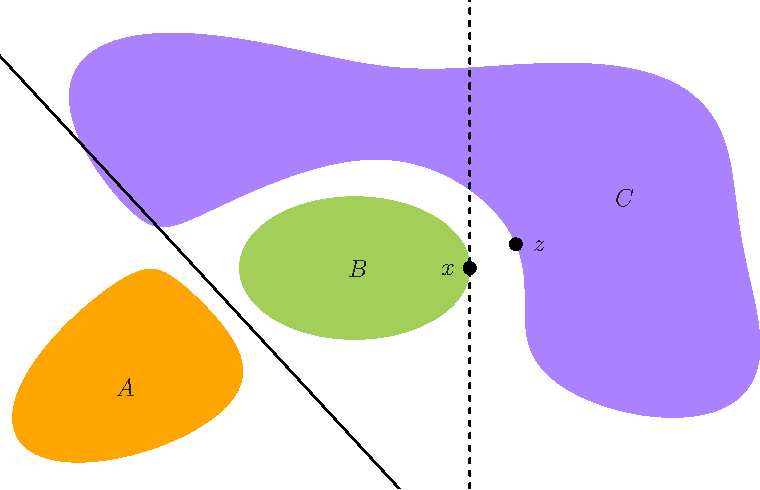
\includegraphics[width=0.675\textwidth]{fig/set_theorems.pdf}
\caption{Lower left, $A$ and $B$: two disjoint convex sets, which must hence 
  admit a separating hyperplane, illustrated as the solid line running between
  them. The set $B$, again by convexity, has a supporting hyperplane at every
  boundary point, illustrated by the dashed line supporting it at $x$. Upper
  right, $B$ and $C$: two disjoint sets which have no separating hyperplane,
  possible because $C$ is nonconvex. The set $C$ has no supporting hyperplane at
  $z$, possible again by nonconvexity.}    
\label{fig:set_theorems}
\end{figure}

\section{Convex functions}
\label{sec:convex_functions}

We now move from sets to functions, which may be a more familiar object of study
to some readers. For reasons that will be apparent, it is convenient to allow
functions to take both real and infinite values. Throughout, by default (without
further specification), a function is defined on all of $\R^d$ and takes values
in the \emph{extended real numbers} $[-\infty, \infty]$. For such $f : \R^d \to
[-\infty, \infty]$, we denote
\index{effective domain}
\[
\dom(f) = \{x : f(x) < \infty \},
\]
and call this set the \emph{effective domain} of $f$. Note that, as we are
allowing functions to take infinite values, there is no loss of generality in
considering functions defined on all of $\R^d$: given $S \subseteq \R^d$ and $f
: S \to [-\infty, \infty]$, we can always be extend $f$ to all of $\R^d$ by
setting it equal to $\infty$ outside of $S$.

We say that $f : \R^d \to (-\infty, \infty]$ is \emph{convex} if $\dom(f)$ is a
convex set and  
\index{convex function} 
\index{strict convexity}
\begin{equation}
\label{eq:convex_function}
f \big(t x + (1-t) y \big) \leq t f(x) + (1-t) f(y),  \quad \text{for all $x,y
  \in \dom(f)$ and $t \in [0,1]$}. 
\end{equation}
This says that the line segment joining $(x,f(x))$ and $(y,f(y))$ lies above  
the graph of $f$, as shown in Figure \ref{fig:convex_function}. We call  
$f$ \emph{strictly convex} provided that strict inequality holds in the above
statement,  
\begin{equation}
\label{eq:strictly_convex_function}
f \big(t x + (1-t) y \big) < t f(x) + (1-t) f(y),  \quad \text{for all $x
  \not= y \in \dom(f)$ and $t \in (0,1)$}. 
\end{equation}
In a sense, this says that $f$ is ``more convex'' than a linear function, as a
linear function would (by definition) have equal left and right hand sides in
\eqref{eq:strictly_convex_function}. A stronger notion than strict convexity is
\emph{strong convexity}, which means, for a parameter $m>0$, the function $f_m$
defined by  
\index{strong convexity}
\[
f_m(x) = f(x) - \frac{m}{2} \|x\|_2^2
\]
is convex. Like strict convexity requires more curvature than a linear function,
strong convexity requires that $f$ be ``more convex'' than a quadratic function. 

A companion notion to convexity is \emph{concavity}. A function $f : \R^d \to  
[-\infty, \infty)$ is called \emph{concave} provided that $-f$ is convex, or
equivalently: $\dom(-f)$ is a convex set and  
\index{concave function} 
\begin{equation}
\label{eq:concave_function}
f \big(t x + (1-t) y \big) \geq t f(x) + (1-t) f(y),  \quad \text{for all $x,y
  \in \dom(-f)$ and $t \in [0,1]$}. 
\end{equation}
Similarly, we say that $f$ is \emph{strictly concave} or \emph{strongly concave}
provided that $-f$ is strictly convex or strongly convex, respectively.   

In general, when it is not clear from the context, we will say that $f$ convex
``on $C$\hspace{1pt}'' to indicate that we are interpreting its effective domain
to be $\dom(f) = C$ (think: we set $f$ to be $\infty$ outside of $C$), and
similarly for concave functions. 

\begin{figure}[tb]
\centering
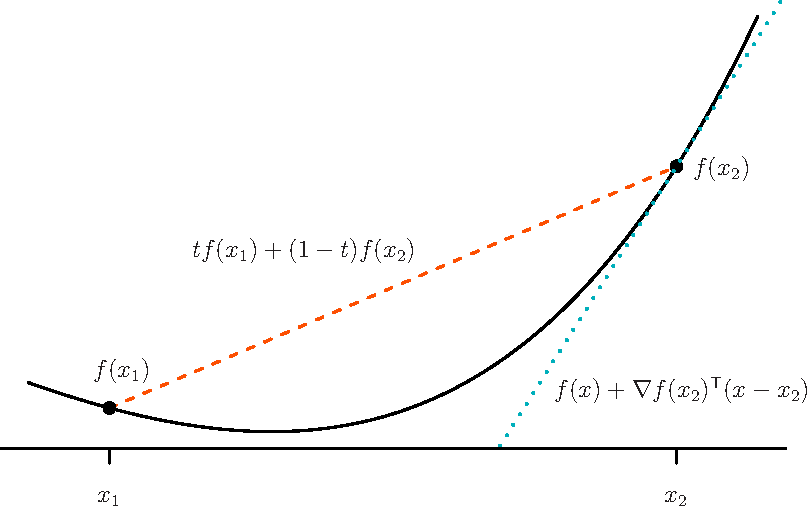
\includegraphics[width=0.7\textwidth]{fig/convex_function.pdf}
\caption{Convex function $f$, such that the line segment between any two points   
  on its graph lies above the function, as illustrated by the dashed line
  joining $(x_1,f(x_1))$ and $(x_2,f(x_2))$. Since $f$ is differentiable,
  convexity is equivalent to $f$ lying everywhere above its tangent line at any
  point, as illustrated by the dotted line running tangent to $f$ at $x_2$.}   
\label{fig:convex_function}
\end{figure}

\begin{Example}
The following are examples of convex or concave functions. In all cases, the
expressions should be interpreted as functions of $x$.

\begin{enumerate}[label=\alph*.]
\item The power function $x^a$ is convex on $\R_+=\{x : x \geq 0\}$ (the
  nonnegative real numbers) for $a \geq 1$, and concave on $\R_{++}= \{x : x > 0\}$
  (the positive real numbers) for $0 < a <  1$. It is also convex on $\R_{++}$
  for $a < 0$.

\item The exponential function $e^x$ is convex on $\R$. The logarithm function
  $\log(x)$ is concave on $\R_{++}$. The \emph{negative entropy} function $x
  \log(x)$ is convex on $\R_{++}$. 
\index{negative entropy function}

\item A linear function $a^\T x + b$ is both convex and concave on $\R^d$. 

\item A quadratic function $\frac{1}{2} x^\T A x + b^\T x + c$ is convex on
  $\R^d$ for $A \succeq 0$ (positive semidefinite) and concave on $\R^d$
  for $A \preceq 0$ (negative semidefinite).

\item A norm $\|x\|$ is always convex. For example, on $\R^d$ we have the
  \emph{$\ell_p$ norms}, defined as: 
  \index{l1 norm@$\ell_1$ norm}
  \index{lp norm@$\ell_p$ norm}
  \index{linf norm@$\ell_\infty$ norm}
  \begin{align}
  \label{eq:lp_norm}
  \|x\|_p &= \bigg(\sum_{i=1}^d |x_i|^p\bigg)^{1/p}, 
  \quad \text{for $p \geq 1$}, \\
  \label{eq:linf_norm}
  \|x\|_\infty &= \max_{i=1,\ldots,d} \, |x_i|,
  \end{align}
  and on $\R^{k \times d}$ we have the \emph{trace norm} and \emph{operator 
    norm}, defined as: 
  \index{trace norm} 
  \index{operator norm}
  \begin{align}
  \label{eq:trace_norm}
  \|X\|_{\tr} &= \sum_{i=1}^k \sigma_i(X), \\
  \label{eq:operator_norm} 
  \|X\|_{\op} &= \sigma_1(X), 
  \end{align}
  respectively (these are also called the \emph{nuclear norm} and \emph{spectral  
    norm}, respectively). Here $\sigma_1(X) \geq \cdots \geq \sigma_k(X) \geq
  0$ denote the singular values of $X$.

\item The \emph{characteristic function} of a set $C$, 
  \index{characteristic function} 
  \begin{equation}
  \label{eq:characteristic_function} 
  I_C(x) = \begin{cases}
  0 & \text{if $x \in C$} \\
  \infty & \text{if $x \notin C$},
  \end{cases}
  \end{equation}
  is convex provided that $C$ is a convex set. 

\item The \emph{support function} of a set $C$, 
  \index{support function}
  \begin{equation}
  \label{eq:support_function}
  h_C(x) = \sup_{z \in C} \, z^\T x,
  \end{equation}
  is always convex (regardless of the set $C$).
\end{enumerate}
\end{Example}

An important property of convex functions is \emph{Jensen's inequality}, which
says that for a convex function $f : \R^d \to (-\infty, \infty]$ and a random 
variable $X$ that is supported on $\dom(f)$, we have     
\index{Jensen's inequality} 
\begin{equation}
\label{eq:jensen}
f( \E[X] ) \leq \E[ f(X) ],
\end{equation}
provided the expectations exist. Oppositely, if $f$ is concave then $f( \E[X]
) \geq \E[ f(X) ]$, again provided the expectations exist. These inequalities
can be seen as generalizations of the defining properties of convexity and
concavity, \eqref{eq:convex_function} and \eqref{eq:concave_function},
respectively, from discrete to arbitrary distributions.

\begin{Remark}
\label{rem:extended_value}
In this book, as per our definitions above, we do \emph{not allow convex
functions to take the value $-\infty$} and do \emph{not allow concave functions
to take the value $\infty$}. This is different from the approach taken by some
other authors and it excludes what are known as \emph{improper} convex functions
from consideration; see the chapter notes for further discussion. Restricting
convex and concave functions in this way will be sufficient for our purposes,
and simplifies matters that would otherwise require a more nuanced treatment.

\setlength{\parindent}{\normalparindent}
To see one advantage of restricting convex functions to take values in
$(-\infty, \infty]$, observe that for $f : \R^d \to (-\infty, \infty]$ with
$\dom(f)$ convex, we can equivalently write \eqref{eq:convex_function} as       
\[
f \big(t x + (1-t) y \big) \leq t f(x) + (1-t) f(y),  \quad \text{for all $x,y
  \in \R^d$ and $t \in [0,1]$}.  
\]
(This is possible because we never encounter the undefined expressions $\infty -
\infty$ or $-\infty + \infty$ in the above statement, as $f$ cannot take the 
value $-\infty$.) This offers an alternative view for convexity, based on
well-defined arithmetic within the extended real numbers, that can be more
fluid when working with functions that can take infinite values.
\end{Remark}

\section{Equivalent characterizations}
\label{sec:equivalent_characterizations}

There are a number of notable alternative characterizations of convexity for
functions (conditions other than the definition that are either equivalent to
convexity or imply convexity), outlined next.  

\paragraph{Epigraph characterization.} 

A function $f : \R^d \to (-\infty, \infty]$ is convex if and only if 
\index{epigraph}
\begin{equation}
\label{eq:epigraph}
\epi(f) = \{ (x,t) \in \dom(f) \times \R : f(x) \leq t \},
\end{equation}
called its \emph{epigraph}, is a convex set. 
  
\paragraph{Lines characterization.} 

A function $f : \R^d \to (-\infty, \infty]$ convex if and only if the
restriction of $f$ to every line is convex, that is, the function $g(t) = f(x +
tv)$ is convex on $\{t : x + tv \in \dom(f)\}$ for all $x,v \in \R^d$.   

\paragraph{First-order characterization.} 

A differentiable function $f : \R^d \to (-\infty, \infty]$ is convex if and only
if $\dom(f)$ is convex and  
\begin{equation}
\label{eq:first_order_characterization}
f(y) \geq f(x) + \nabla f(x)^\T (y-x), \quad \text{for all $x,y \in \dom(f)$},  
\end{equation}
where $\nabla f(x)$ denotes the gradient of $f$ at $x$. This says that
first-order Taylor approximation to $f$ around any point $x$ must
globally under-approximate $f$; this is illustrated in Figure
\ref{fig:convex_function}. A similar result holds for strict convexity: a
differentiable function $f : \R^d \to (-\infty, \infty]$ is strictly convex if
and only if $\dom(f)$ is convex and 
\[
f(y) > f(x) + \nabla f(x)^\T (y-x), \quad \text{for all $x \not= y \in
  \dom(f)$}.   
\]
 
\paragraph{Second-order characterization.} 

A twice differentiable function $f : \R^d \to (-\infty, \infty]$ is convex if
and only if $\dom(f)$ is convex and  
\begin{equation}
\label{eq:second_order_characterization}
\nabla^2 f(x) \succeq 0, \quad \text{for all $x \in \dom(f)$},
\end{equation}
where $\nabla^2 f(x)$ denotes the Hessian of $f$ at $x$. This condition says
that the function $f$, at any point $x$, must be ``curved upwards'' in any
direction; more precisely, for $v \in \R^d$, letting $g(t)=f(x+tv)$, we see
that $g''(0) = v^\T \nabla^2 f(x) v \geq 0$ (by positive semidefiniteness). For
twice differentiable $f : \R^d \to (-\infty, \infty]$, if $\dom(f)$ is convex
and     
\[
\nabla^2 f(x) \succ 0, \quad \text{for all $x \in \dom(f)$},
\]
meaning $\nabla^2 f(x)$ is positive definite for all $x \in \dom(f)$, then $f$
is strictly convex. However, we note that this is \emph{not} a necessary   
condition; for example, $f(x) = x^4$ is strictly convex but $f''(0)=0$. 

\medskip

For concavity, each of the above equivalent characterizations has an analog
(we just apply the characterization to $-f$). For alternative
characterizations of strong convexity, see Theorem \ref{thm:strong_convexity}. 

\begin{Example} 
The convexity or concavity of the following two functions can be confirmed
using the second-order characterization
\eqref{eq:second_order_characterization}. 

\begin{enumerate}[label=\alph*.]
\item The \emph{log-sum-exp function}, defined by 
  \index{log-sum-exp function} 
  \[
  f(x) = \log\bigg( \sum_{i=1}^d e^{x_i} \bigg),
  \]
  is convex on $\R^d$.

\item The \emph{log-det function}, defined by $f(X) = \log(\det(X))$, is concave
  on $\SS_{++}^d = \{X \in \SS^d : X \succ 0\}$ (the space of positive definite
  $d \times d$ matrices). 
  \index{log-det function} 
\end{enumerate}
\end{Example}

\section{Operations preserving convexity}
\label{sec:operations_preserving_convexity}

To check the convexity of a given set or function, we can of course apply the
definition directly, or for functions, we can appeal to the alternative
characterizations from Chapter \ref{sec:equivalent_characterizations}. For
complicated sets or functions, this can become tedious. It is often easier to
instead (a) memorize a few key base examples of convex sets and functions (for
example, those given in Chapters \ref{sec:convex_sets} and
\ref{sec:convex_functions}), and (b) remember that various transformations
preserve convexity (as we will detail below). Then, checking convexity for a
given set or function becomes a task of trying to relate it to one of the key
base examples by one (or any sequence of) convexity-preserving transformations.

Here are some useful operations that preserve convexity for sets.

\paragraph{Intersection.} 
\parlab{par:set_intersection} 

If $C_s$ is convex for each $s \in S$, then the intersection \smash{$\cap_{s \in
    S} \, C_s$} is convex. 

\paragraph{Scaling and translation.} 

If $C \subseteq \R^d$ is convex, $a \in \R$, and $b \in \R^d$, then 
\[
aC+b = \{ ax + b : x \in C \}
\]
is convex.

\paragraph{Linear images and preimages.} 
\parlab{par:set_linear}

If $C \subseteq \R^d$ is convex and $f(x)=Ax+b$ for $A \in \R^{k \times d}$ and
$b \in \R^k$, then the image of $C$ under $f$, 
\[
f(C) = \{ f(x) : x \in C \}
\]
is convex. Also, if $D \subseteq \R^k$ is convex, then the preimage (or
inverse image) of $D$ under $f$,  
\[
f^{-1}(D) = \{ x : f(x) \in D \}
\]
is convex.

\paragraph{Perspective images and preimages.} 

The $(d+1)$-variate \emph{perspective function} is defined for $x \in \R^d$ and
$z>0$ as   
\index{perspective function}
\[
P(x,z) = x/z.
\]
Note $\dom(P)=\R^d \times \R_{++}$ (where recall $\R_{++}$ denotes the    
positive reals). If $C \subseteq \dom(P)$ is convex then the perspective image
$P(C)$ is convex; and if $D \subseteq \R^d$ is convex then the perspective
preimage $P^{-1}(D)$ is convex.  

\paragraph{Linear-fractional images and preimages.} 

A \emph{linear-fractional function} is the composition of a perspective function
with a linear function, that is, a function $f$ of the form      
\index{linear-fractional function} 
\[
f(x) = \frac{Ax + b}{c^\T x + e},
\]
with $\dom(f) = \{x : c^\T x + e > 0\}$. Supposing that $A \in \R^{k
  \times d}$, if $C \subseteq \R^d$ is convex and $C \subseteq \dom(f)$ then 
the linear-fractional image $f(C)$ is convex; and if $D \subseteq \R^k$ is 
convex then the linear-fractional preimage $f^{-1}(D)$ is convex.

\medskip

Here are now some useful operations that preserve convexity for functions (note
the analogy to the operations for sets, in many cases). 

\paragraph{Nonnegative linear combination.} 

If $f_1,\ldots,f_n$ are convex functions and $a_1,\ldots,a_n \geq 0$ then the
nonnegative linear combination $F = a_1f_1+\cdots+a_nf_n$, the function defined
as
\[
F(x) = a_1f_1(x) + \cdots + a_nf_n(x) 
\]
is convex.

\paragraph{Partial supremum.} 
\parlab{par:function_supremum}

Let $f$ be a function acting on a block variable $(x,z)$. If $f(\cdot,z)$ is
convex for each $z \in Z$ (meaning, $x \mapsto f(x,z)$ is convex), then the
partial supremum \smash{$F = \sup_{z \in Z} f(\cdot,z)$}, the function defined
as  
\index{partial supremum!convexity}
\[
F(x) = \sup_{z \in Z} \, f(x,z),
\]
is convex. An important special case, corresponding to a finite set $Z$: if
$f_i$, $i=1,\ldots,k$ are convex, then their pointwise maximum $F$, defined as
\smash{$F(x) = \max_{i=1,\ldots,k} \, f_i(x)$}, is convex.      

\paragraph{Partial infimum.} 
\parlab{par:function_infimum}

Let $f$ be a function acting on a block variable $(x,z)$. If $f$ is convex (to
be clear and to emphasize the difference to the above, here we mean $(x,z)
\mapsto f(x,z)$ is convex) and $Z$ is a convex set, then the partial infimum
\smash{$F = \inf_{z \in Z} f(\cdot,z)$}, the function defined as  
\index{partial infimum!convexity}
\[
F(x) = \inf_{z \in Z} \, f(x,z),
\]
is convex, provided that $F$ is nowhere equal to $-\infty$. 

\paragraph{Linear composition.} 
\parlab{par:function_linear}

Let $f : \R^k \to (-\infty, \infty]$ be convex, and let $A \in \R^{k \times d}$,
$b \in \R^d$. Then the function $F$ defined as $F(x) = f(Ax+b)$ is convex.     

\paragraph{Perspective transformation.} 
\parlab{par:function_perspective}

The \emph{perspective transform} of $f$ is the function defined as
\index{perspective transform}
\[
F(x,t) = t f(x/t),
\]
with $\dom(F) = \dom(f) \times \R_{++}$. If $f$ is convex, then so is its
perspective transform. 

\paragraph{General composition.} 
\parlab{par:function_composition}

Let $f : \R^k \to (-\infty, \infty]$, $g : \R^d \to \R^k$, and denote their
composition by $F = f \circ g$, that is, $F(x) = f(g(x))$. Then $F$ is convex if
$f$ is convex and, for each $i=1,\ldots,k$, either of the following holds (where
$g_i$ denotes the $i\th$ component function of $g$): 
\index{composition!convexity}
\begin{itemize}
\item $f$ is nondecreasing in its $i\th$ argument and $g_i$ is convex; or
\item $f$ is nonincreasing in its $i\th$ argument and $g_i$ is concave.
\end{itemize} 

To develop intuition for this rule, it helps to think of univariate twice
differentiable $f,g$ (though the rule of course applies more generally). In this
case, we can use the chain rule to compute
\[
F''(x) = f''(g(x)) (g'(x))^2 + f'(g(x)) g''(x).
\]
In order to have $F'' \geq 0$, we see that it suffices to have $f'' \geq 0$ and
$g'' \geq 0$ (that is, $f$ and $g$ convex) as well as $f' \geq 0$ (that is, $f$
nondecreasing). It would also work to have $f'' \geq 0$ and $g'' \leq 0$ (that
is, $f$ convex and $g$ concave) as well as $f' \leq 0$ (that is, $f$
nonincreasing).

\medskip

\begin{Example}
The following claims about convexity can be checked by identifying   
the right base examples and convexity-preserving transformations. 

\begin{enumerate}[label=\alph*.]
\item For $A_1,\ldots,A_d,B \in \SS^n$, the set $\{x : x_1 A_1 + x_2 A_2 +
  \cdots + x_d A_d \preceq B \}$ is convex.  

\item For $C \subseteq \R^d$ and a norm $\|\cdot\|$, the function giving the
  supremum distance to $C$,
\[
f(x) = \sup_{z \in C} \, \|x - z\|,
\]
is convex.

\item For $C \subseteq \R^d$ and a norm $\|\cdot\|$, the function giving the
  infimum distance to $C$,
\[
f(x) = \inf_{z \in C} \, \|x - z\|,
\]
is convex, provided that $C$ is convex.
\end{enumerate}
\end{Example}

Many common loss functions in statistical estimation and machine learning are
convex, and this can be readily checked using the results from this section or
the last; see Exercise \ref{ex:loss_functions}.             

\section{Equivalent growth conditions*}

We say that a function $F$ is \emph{Lipschitz continuous} with parameter $L>0$
if 
\index{Lipschitz continuity}
\index{Lipschitz smoothness}
\[
\|F(x) - F(y)\|_2 \leq L \|x-y\|_2, \quad \text{for all $x,y \in
  \dom(f)$}. 
\]
We say that a function $f$ is \emph{Lipschitz smooth} with parameter $L>0$
provided $f$ is differentiable and its gradient $F=\nabla f$ satisfies the above
condition. 

Lipschitz continuity can be seen as a type of growth condition on the function
in question. To develop intuition for this, consider the case of a real-valued
function $F$: Lipschitz continuity means that, along any line segment, $F$
cannot grow faster than a linear function with slope $L$. Thus for real-valued $f$,
when $\nabla f$ is Lipschitz continuous ($f$ is Lipschitz smooth), one might
imagine that $f$ cannot grow faster than a quadratic function. The next
result makes this precise, and provides several other conditions related to
Lipschitz smoothness.

\index{Lipschitz smoothness}
\begin{Theorem}
\label{thm:lipschitz_smoothness}
For differentiable $f : \R^d \to (-\infty, \infty]$ and $L>0$, consider the
statements:  
\begin{enumerate}[label=(\roman*)]
\item $\|\nabla f(x) - \nabla f(y)\|_2 \leq L \|x-y\|_2$, for all $x,y \in
  \dom(f)$; 
\item the function $-f_L$ is convex, where $f_L(x) = f(x) - \frac{L}{2}
  \|x\|_2^2$;   
\item $f(y) \leq f(x) + \nabla f(x)^\T (y-x) + \frac{L}{2} \|y-x\|_2^2$, for all
  $x,y \in \dom(f)$;
\item $(\nabla f(x) - \nabla f(y))^\T (x - y) \leq L\|x-y\|_2^2$, for all $x,y
  \in \dom(f)$.
\end{enumerate}
Then the following relations hold: 
\[
\text{(i)} \implies \text{(ii)} \iff \text{(iii)} \iff \text{(iv)}. 
\]
If $f$ is twice continuously differentiable, then (ii)--(iv) are also equivalent
to the statement: 
\begin{enumerate}
\item[(v)] $\nabla^2 f(x) \preceq LI$, for all $x \in \dom(f)$.
\end{enumerate} 
Lastly, for convex $f$, statements (i)--(iv) are all equivalent, and for twice  
continuously differentiable convex $f$, statements (i)--(v) are all equivalent. 
\end{Theorem}

Interestingly, the concept of strong convexity admits a similar string of
equivalences. 

\index{strong convexity}
\begin{Theorem}
\label{thm:strong_convexity}
For differentiable $f : \R^d \to (-\infty, \infty]$ and $m>0$, consider the
statements:  
\begin{enumerate}[label=(\roman*)]
\item $\|\nabla f(x) - \nabla f(y)\|_2 \geq m \|x-y\|_2$, for all $x,y \in
  \dom(f)$; 
\item the function $f_m$ is convex, where $f_m(x) = f(x) - \frac{m}{2}
  \|x\|_2^2$;   
\item $f(y) \geq f(x) + \nabla f(x)^\T (y-x) + \frac{m}{2} \|y-x\|_2^2$, for all
  $x,y \in \dom(f)$;
\item $(\nabla f(x) - \nabla f(y))^\T (x - y) \geq m\|x-y\|_2^2$, for all $x,y
  \in \dom(f)$.
\end{enumerate}
Then the following relations hold: 
\[
\text{(i)} \impliedby \text{(ii)} \iff \text{(iii)} \iff \text{(iv)}. 
\]
If $f$ is twice continuously differentiable, then (ii)--(iv) are also equivalent
to the statement: 
\begin{enumerate}
\item[(v)] $\nabla^2 f(x) \succeq mI$, for all $x \in \dom(f)$.
\end{enumerate}
\end{Theorem}

Comparing Theorems \ref{thm:lipschitz_smoothness} and
\ref{thm:strong_convexity}, we might view Lipschitz smoothness and strong
convexity as dual concepts, informally speaking, since they give rise to
conditions that are symmetric in nature. (Perhaps not surprisingly, the proofs
of these conditions also proceed symmetrically, as outlined in Exercise
\ref{ex:lipschitz_smoothness}.)  In fact, as we will see later in Chapter 
\ref{sec:conjugate_smoothness}, there is a deeper (formal) dual relation at
play: Lipschitz smoothness of a function is intimately tied to strong convexity
of its conjugate.

\section{Smoothness properties*}

Much of this chapter studies convex functions through the lens of their
gradients (or Hessians). Of course, a convex function need not be differentiable
(or twice differentiable); the function $f(x) = |x|$, for example, is convex but
not differentiable at $x=0$. Meanwhile, if we stick to the univariate case,
then it seems intuitively that for a convex function the only possibilities for 
nondifferentiability are ``kink'' points, like the behavior of the absolute
value function at the origin. This leads us to wonder: to what extent can a
convex function lack smoothness in general? Can it be arbitrarily nonsmooth, or 
does convexity itself impose restrictions on how ``much'' nonsmootheness is
permitted? The next theorem answers these questions.

\index{Lipschitz smoothness} 
\index{Rademacher's theorem} 
\index{Aleksandrov's theorem} 
\begin{Theorem} 
\label{thm:smoothness_properties}
Let $f$ be a convex function. Then the following hold: 
\begin{enumerate}[label=(\roman*)]
\item $f$ is continuous at every point in $\interior(\dom(f))$;
\item in fact, $f$ is locally Lipschitz continuous on $\interior(\dom(f))$,
  meaning that for each compact set $C \subseteq \interior(\dom(f))$, there
  is a constant $L>0$ (this can depend on $C$) such that        
  \[
  |f(x) - f(y)| \leq L \|x-y\|_2, \quad \text{for all $x,y \in C$};
  \]
\item hence, $f$ is differentiable at almost every point in
  $\interior(\dom(f))$;   
\item moreover, $f$ is twice differentiable at almost every point in 
  $\interior(\dom(f))$.  
\end{enumerate}
\end{Theorem}

We remark that property (i) actually holds at every point in
$\relint(\dom(f))$,\footnote{The precise statement here is that the restriction
  of $f$ to $\relint(\dom(f))$ is continuous; that is, for each $x \in
  \relint(\dom(f))$, we have \smash{$\lim_{k \to \infty} f(x_k) \to f(x)$}
  whenever \smash{$\lim_{k \to \infty} x_k= x$} and \smash{$\{x_k\}_{k=1}^\infty
    \subseteq \relint(\dom(f))$}.} 
and we only write $\interior(\dom(f))$ in the theorem statement theorem to
preserve symmetry in the presentation of (i)--(iv). We also remark that property 
(iii) follows from (ii): that locally Lipschitz functions are differentiable
almost everywhere is a result known as \emph{Rademacher's theorem}. Property
(iv), the almost everywhere twice differentiability of convex functions, is
known as \emph{Aleksandrov's theorem}. To be explicit, when we say that a
certain property holds for almost every point in a set $S$, we mean that it
holds on a set $E \subseteq S$ such that $S \setminus E$ has Lebesgue measure
zero.

% Continuity: for example, Theorem 10.1 in Rockafellar (1970)
% Local Lipschitz: for example, Theorem 6.7 in Evans & Gariepy (2015) 
% Differentiability: for example, Theorem 6.6 in Evans & Gariepy (2015) 
% Twice differentiability: for example, Theorem 6.9 in Evans & Gariepy (2015) 
% Continuous differentiability (not relayed here): for example, Theorem 25.5 in
% Rockafellar (1970)?  

While the almost everywhere differentiability and twice differentiability of
convex functions is quite remarkable, we should be mindful to not overinterpret
the implications of Theorem \ref{thm:smoothness_properties}, as they pertain to
convex optimization. Generally speaking, sets of Lebesgue measure zero cannot be
ignored in mathematical optimization (unlike, say, functional analysis),
particularly because many optimization problems of interest lack smoothness at
their minima; when this happens, as we will see in the subsequent chapters, we
must account for it, both analytically and algorithmically, and subgradients
will be one of our main tools for doing so.

\section{Cones and polyhedra*}
\label{sec:cones_polyhedra}

We cover cones and polyhedra in a bit more detail, two classes of sets that 
have special structure and play a central role in convex optimization. 

\subsection{Cones}
\label{sec:cones}

A set $C \subseteq \R^d$ is called a \emph{cone} if it satisfies 
\index{cone} 
\begin{equation}
\label{eq:cone}
x \in C \implies t x \in C, \quad \text{for all $t \geq 0$}.
\end{equation}
A special type of cone of particular interest is a \emph{convex cone}, which is
simply a set that is both a cone and convex. Combining \eqref{eq:convex_set} and
\eqref{eq:cone}, we see that a convex cone $C$ is defined by 
\index{convex cone}  
\begin{equation}
\label{eq:convex_cone}
x, y \in C \implies s x + t y \in C, \quad \text{for all $s, t \geq 0$}.
\end{equation}
Recall that the positive semidefinite cone \eqref{eq:psd_cone} and normal cone
\eqref{eq:normal_cone} are both convex cones. Another noteworthy example
is the \emph{norm cone}, defined for a norm $\|\cdot\|$ by 
\index{norm!cone}  
\begin{equation}
\label{eq:norm_cone}
\{ (x,t) \in \R^d \times \R : \|x\| \leq t \}.
\end{equation}

The \emph{conic hull} of $C$ is the set of all nonnegative linear combinations
of points in $C$,   
\[ 
\cone(C) = \bigg\{
\sum_{i=1}^n t_i x_i : 
\text{$n \geq 1$, $x_i \in C$, $t_i \geq 0$, for $i=1,\ldots,n$} \bigg\}. 
\]
The conic hull $\cone(C)$ is itself a convex cone, for any set $C$; in fact, it
is the smallest convex cone containing $C$, meaning that $\cone(C) \subseteq D$ 
for any convex cone $D \supseteq C$. 

Next we present a classical result on conic and convex hulls.

\index{Carath\'{e}odory's theorem}
\begin{Theorem}[Carath\'{e}odory's theorem]
\label{thm:caratheodory}
Let $C \subseteq \R^d$.

\begin{enumerate}[label=(\roman*)]
\item Every nonzero element in the conic hull $\cone(C)$ can be represented as a
  positive linear combination of linearly independent (and thus at most $d$)
  elements of $C$.  

\item Every element in the convex hull $\conv(C)$ can be represented as a convex
  combination of affinely independent (and thus at most $d+1$) elements of $C$.  
\end{enumerate}
\end{Theorem}

% Note: typical proof of convex hull result, using conic hull result, implies
% affine independence (though this isn't typically stated)

This has various important implications; see part f of Exercise
\ref{ex:convex_closed} for a basic one. 

\subsection{Polyhedra}
\label{sec:polyhedra}

A \emph{polyhedron} $P \subseteq \R^d$ is the intersection of a finite number of
halfspaces, which we can express generically as 
\index{polyhedron}
\[
P = \{x : Ax \leq b\}
\] 
for a matrix $A$ and vector $b$, where recall we interpret this inequality
componentwise. It should be clear that $\{x : Ax \geq b\}$, $\{x : \ell \leq Ax
\leq u\}$, and $\{x : Ax \leq b, \, Gx = h\}$ are all also polyhedra, as we
can rewrite each of them in the form of the above display, for appropriately
(re)defined $A,b$.

Less obvious is the fact that an optimization problem over a polyhedron can
always be equated with a higher-dimensional optimization problem over the
intersection of an affine subspace and the nonnegative orthant, $\{x : Ax=b, \,
x \geq 0 \}$. We will revisit this when we discuss linear programs in standard
form, in Chapter \ref{sec:linear_programs}. 

We call a bounded polyhedron a \emph{polytope}. A fundamental fact about
polytopes is as follows. 
\index{polytope} 

\begin{Theorem}
\label{thm:v_representation}
Every polytope can be represented as the convex hull of a finite set of points. 
\end{Theorem}

% For example, Theorem 3 page 32 in Grunbaum (2003)

This result is both highly intuitive and highly nontrivial; later, in Chapter
\ref{sec:dual_cones_polar_sets}, we will return to it from the perspective of
duality. Now we simply introduce some nomenclature to help
remember Theorem \ref{thm:v_representation}: we call $P = \{x : Ax \leq
b\}$ a \emph{halfspace representation} or \emph{H-representation} of $P$, and $Q
=  \conv\{x_1,\ldots,x_n\}$ a \emph{vertex representation} or  
\emph{V-representation} of $Q$. Then in this language, the theorem 
says that every polytope has an equivalent H-representation and
V-representation.   

An interesting aspect of polyhedra is their facial structure. A \emph{face} $F$
of a polyhedron $P \subseteq \R^d$ is a set $F$ such that 
\index{polyhedron!face}
\index{polyhedron!vertex}
\index{convex set!exposed point}  
\[
\text{$F = \emptyset$, $F = P$, or $F = P \cap H$ for a supporting hyperplane
  $H$ of $P$}. 
\]
The faces $F=\emptyset$ and $F=P$ are said to be \emph{improper}; each other
face of $F$ of $P$ is called \emph{proper}. A face $F$ is said to have dimension
$k$ (or, called a $k$-face) if its affine span $\aff(F)$ is $k$-dimensional. A
maximal proper face (proper face of maximum degree) of $P$ is called a
\emph{facet} of $P$. If $F=\{x\}$ is a $0$-face of $P$, then we call $x$ an
\emph{vertex} of $P$. 

To be fair, these concepts are not specific to polyhedra and the same
definitions apply to convex sets in general. A small difference in
nomenclature: if $F = \{x\}$ is a $0$-face of a convex set $C$, then we call $x$
an \emph{exposed point} of $C$ (for polyhedra, vertices and exposed points 
are equivalent, but not in general). Even in the general convex setting, these
concepts lead to interesting developments; for example, for any compact (closed
and bounded) convex set $C$, 
\index{Straszewicz' theorem}   
\[
C = \closure\big(\conv\{x : \text{$x$ is an exposed point of $C$}\}\big),  
\]
% For example, Theorem 8 page 19 in Grunbaum (2003) 
a result called \emph{Straszewicz' theorem}. (For polytopes, the above is true
without the surrounding $\closure(\cdot)$ because the set of exposed
points---that is, the vertex set---is finite.) For more, see Exercise
\ref{ex:extreme_points}. 

What makes polyhedra so special, however, is the \emph{structure} exhibited by
their faces. The faces of a polyhedron $P$ obey a beautiful recursive 
structure: each face of a face of $P$ is also a face of $P$, each face of $P$
can be expressed as an intersection of facets of $P$, and so on. 
% For example, Theorem 1 page 26 and Theorem 5 page 27 in Grunbaum (2003) 
We will not go into this in any detail, but we will leverage the relationship
between faces of $P$ and faces of its dual polytope $P^*$ when we prove
Theorem \ref{thm:v_representation} in Chapter \ref{sec:dual_cones_polar_sets}. 

\SkipTocEntry\section*{Chapter notes}

There is a lot to be said about convex sets and functions, far more than what is
said in this chapter. For readers seeking a more in-depth treatment, there are
many excellent references on the subject, for example,
\cite{rockafellar1970convex} (Chapters 1--11, 17--22),
\cite{hiriartUrruty2001fundamentals} (Chapters A, B), \cite{boyd2004convex}
(Chapters 2, 3), \cite{bertsekas2009convex} (Chapters 1, 2), to name just a
few. For more details on operations that preserve convexity, we refer readers to 
\cite{boyd2004convex} (Chapters 2.3, 3.2). For greater depth on the smoothness
properties of convex functions, we refer to \cite{rockafellar1970convex}
(Chapters 10, 25), or \cite{evans2015measure} (Chapters 6.3, 6.4). To learn more
about polyhedra and their structure, a classic reference is
\cite{grunbaum2003convex}.  

As briefly discussed in Remark \ref{rem:extended_value}, our definition of a
convex function does not allow it to take the value $-\infty$ (and likewise, we
do not allow a concave function to take the value $\infty$). This is in
contradiction with the standard approach in convex analysis, for example
\cite{rockafellar1970convex, bertsekas2009convex} (but it is consistent with 
the approach of others, for example \cite{boyd2004convex}). The standard
approach in convex analysis allows a convex function to take values in
$[-\infty,\infty]$, and defines a \emph{proper} convex function $f$ as one
such that $f \not= \infty$ and $f > -\infty$ ($f$ is not identically $\infty$,
and never $-\infty$). While proper convex functions are the real topic of
interest, \emph{improper} convex functions do arise in various situations, and
there are some nontrivial improper convex functions that are not just
identically $\pm \infty$, for example
\[
f(x) = \begin{cases}
-\infty & \text{if $\|x\| < 1$} \\
0 & \text{if $\|x\| = 1$} \\
\infty & \text{if $\|x\| > 1$},
\end{cases}
\]
for a norm $\|\cdot\|$. Thus, from a general mathematical perspective, it is
important to be able to deal with them. Altogether, for our purposes, we find it
simpler to rule them out completely, though we admit this does come with its own
set of drawbacks, for example we must occasionally add explicit qualifiers to
statements about certain functions lying above $-\infty$, as we did in Property 
\parref{par:function_infimum}, the convexity-preserving rule for a partial
infimum.

\clearpage

\begin{xcb}{Exercises}
\begin{enumerate}[label=\thechapter.\arabic*]
\settowidth{\leftmargini}{0.00.\hskip\labelsep}
\item Prove that if $X$ is a random variable supported on a convex set $C
  \subseteq \R^d$ (and $\E(X)$ exists) then $\E(X) \in C$.  

\item \label{ex:convex_sublevel}
  Show that if $f$ is a convex function, then $\{x : f(x) \leq t \}$, called the
  \emph{sublevel set} of $f$ at level $t$, is a convex set. Show that the
  converse is not true: give an example of a nonconvex function whose sublevel
  sets are convex (for all levels $t$).

\item \label{ex:convex_closed}
  We explore some of the differences between preserving convexity and closedness
  of sets. 

\begin{enumerate}[label=\alph*.]
\item Prove Property \parref{par:set_intersection}, that an intersection of
  (any number of) convex sets is convex.

\item Prove that the intersection of (any number of) closed sets is closed.

\item Prove Property \parref{par:set_linear}, that linear images and preimages
  of convex sets are convex. 

\item Show that the preimage of a closed set under a linear map is closed; but
  the image of a closed set under a linear map need not be closed (give a
  counterexample). 

\index{convex hull}
\item Give an example of a closed set whose convex hull is not closed. 
  
\index{Carath\'{e}odory's theorem}
\item Prove that the convex hull of a compact (closed and bounded) set is
  compact. Hint: use part (ii) of Carath\'{e}odory's theorem (Theorem
  \ref{thm:caratheodory}), and sequential compactness.   
\end{enumerate}

\item \label{ex:convex_flavors}
  We explore some properties of the various ``flavors'' of convexity.   

\begin{enumerate}[label=\alph*.]
\index{strict convexity}
\item Give an example of a strictly convex function that is not strongly
  convex. 
  
\index{strong convexity}
\item Give an example of a strongly convex function that is not differentiable. 

\item Give an example of a strictly convex function $f$ such that $f(x) \to
  -\infty$ as $\|x\|_2 \to \infty$. 

\item Prove that for any differentiable strongly convex function $f$, we must
  have $f(x) \to \infty$ as $\|x\|_2 \to \infty$. Hint: use part (iii) of Theorem
  \ref{thm:strong_convexity}.
  
  \smallskip
  Note: differentiability is not actually required here; strong convexity alone
  is enough as we can use part (iii) of Theorem
  \ref{thm:strong_convexity_nonsmooth}; see Exercise
  \ref{ex:strong_convexity_coercive}.  
\end{enumerate}

\index{composition!convexity}
\item \label{ex:function_composition} 
  We explore Property \parref{par:function_composition} from a few perspectives.   

\begin{enumerate}[label=\alph*.]
\item Prove Property \parref{par:function_composition} by verifying directly
  that $F$ satisfies the definition of convexity. 

\item Prove that the second bullet point in Property
  \parref{par:function_composition} can be collapsed into the first: if the
  conditions stated in the property hold, and there exists $i$ such that $f$ 
  nonincreasing in its $i\th$ argument and $g_i$ concave, then we can
  reparametrize by flipping the signs of the appropriate arguments/component 
  functions, and thus we can write \smash{$F = \tilde{f} \circ \tilde{g}$} for  
  \smash{$\tilde{f}$} nondecreasing in each argument and \smash{$\tilde{g}$} 
  having all component functions convex. 

\item Prove that Property \parref{par:function_composition} can be extended to
  the case where $g$ takes infinite values, in the following way. If $f : \R^k
  \to (-\infty, \infty]$ is convex and nondecreasing in each argument, and $g :
  \R^d \to (-\infty, \infty]^k$ is convex in each component, then $F = f \circ
  g$ is convex, where we set $F(x) = \infty$ for any $x$ with at least one
  component equal to $\infty$.  
\end{enumerate}

\item \label{ex:loss_functions} 
  In this exercise, we practice checking convexity, focusing on functions that 
  commonly appear in statistical estimation and machine learning. In some 
  instances, it might be easiest to use convexity-preserving operations from 
  Chapter \ref{sec:operations_preserving_convexity}, in others, it might be
  easier to prove the given claim straight from the definition.

\begin{enumerate}[label=\alph*.]
\index{linear regression}
\item \emph{Linear regression loss.} Prove that $f(\beta) = \|y -
  X \beta\|_2^2$ is convex, for any $X \in \R^{n \times d}$ and $y \in \R^n$.  

\index{logistic regression}
\item \emph{Logistic regression loss.} Prove that \smash{$f(\beta) = -y^\T 
    X \beta + \sum_{i=1}^n \log(1+e^{x_i^\T \beta})$} is convex, for any $X \in 
  \R^{n \times d}$ and $y \in \{0,1\}^n$, where $x_i \in \R^d$, $i=1,\ldots,n$  
  denote the rows of $X$.
  
\item \emph{Hinge classification loss.} Prove that \smash{$f(\beta) =
    \sum_{i=1}^n (1 - y_i x_i^\T \beta)_+$} is convex, where $a_+ = \max\{a,
  0\}$, for any $x_i \in \R^d$, $i=1,\ldots,n$ and $y \in \{-1,1\}^n$, 

\item \emph{Kullback-Leibler divergence between discrete distributions.} Prove
  that 
  \index{Kullback-Leibler divergence} 
  \[
  f(p,q) = \sum_{i=1}^d p_i \log(p_i / q_i) 
  \]
  is a convex function of $(p,q) \in \{ x \in \R^{2d} : \one^\T x = 1, \, x >
  0\}$.

\item \emph{Gaussian log likelihood for precision matrix.} Prove that 
  \index{Gaussian likelihood}
  \[
  f(\Sigma^{-1}) = -\frac{n}{2} \log(\det(\Sigma)) - \frac{1}{2} \sum_{i=1}^n 
  (x_i-\mu)^\T \Sigma^{-1} (x_i-\mu)
  \]
  is a concave function of $\Sigma^{-1} \in \SS_{++}^d$ (the inverse
  covariance matrix, called the \emph{precision matrix}), for any $x_i \in
  \R^d$, $i=1,\ldots,d$ and $\mu \in \R^d$. Hint: use the relationship between
  $\det(A)$ and $\det(A^{-1})$ for an invertible matrix $A$, and also linearity
  of the trace operator $\tr(\cdot)$. 

\item Let $f$ be strictly convex with $\dom(f)=\R^d$. By Property
  \parref{par:function_linear}, the linear composition rule, we know that  
  $g(\beta) = f(X \beta)$ is convex for any $X \in \R^{n \times d}$. Prove 
  that $g$ is strictly convex if and only if $\rank(X)=d$. 
\end{enumerate}

\item Now we practice checking nonconvexity. In some cases, a counterexample to
  \eqref{eq:convex_function} should be simple to produce; in others, inspecting
  the second-order condition \eqref{eq:second_order_characterization} might be
  easier.  

\begin{enumerate}[label=\alph*.]
\item \emph{$\ell_0$ ``norm''.}  Prove that $f(x) = \|x\|_0$, where
  \index{l0 norm@$\ell_0$ norm}
  \begin{equation}
  \label{eq:l0_norm}
  \|x\|_0 = \sum_{i=1}^d 1\{x_i \not= 0\}
  \end{equation}
  is the $\ell_0$ ``norm'', is nonconvex over $\R^d$.

  \smallskip
  Note: we use quotation marks since $\|\cdot\|_0$ is not a norm (it lacks
  positive homogeneity) and calling it a \emph{pseudonorm} would be more
  appropriate; however, we adopt the common terminology henceforth and simply
  refer to it as a norm (without quotations).   

\item \emph{Matrix rank.} Prove that $f(x) = \rank(X)$ is nonconvex over $\R^{n
    \times d}$.   

\item \emph{Gaussian negative log likelihood for mean and variance.} Prove that  
  \[
  f(\mu, \sigma^2) = \log \sigma + \frac{(y - \mu)^2}{2\sigma^2}
  \]
  is nonconvex over $\R \times \R_{++}$.

\item \emph{Least squares for two-layer neural network.} Prove that 
  \index{neural network}
  \[
  f(W, u, v) = \sum_{i=1}^n \bigg( y_i - \sum_{j=1}^k v_j 
  \phi (w_j^\T x_i + u_j) \bigg)^2 
  \]
  is nonconvex over $\R^{k \times p} \times \R^k \times \R^k$, where $\phi : \R
  \to \R$ can be taken (for simplicity) to be twice differentiable and monotone.    
\end{enumerate}

\item \label{ex:farkas} 
  The following is a ``strict'' variant of the separating hyperplane theorem: if 
  $C,D$ are nonempty disjoint closed convex sets, and (say) $D$ is bounded, 
  then there exists $a \not=0 $ and $b$ such that 
  \index{separating hyperplane theorem!strict version}
  \[
  \text{$a^\T x > b$ for all $x \in C$ and $a^\T x < b$ for all $x \in D$},
  \]  
  % For example, see proof in Section 2.5.1 of Boyd & Vandenberghe (2004)
  that is, the hyperplane $\{x: a^\T x =  b\}$ strictly separates $C,D$. 
  Use this to prove \emph{Farkas' lemma}: given $A \in \R^{k \times d}$, $b \in 
  \R^k$, exactly one of the following statements is true: 
  \index{Farkas' lemma} 
  \begin{itemize}
  \item there exists $x \in \R^d$ such that $Ax=b$, $x \geq 0$;
  \item there exists $y \in \R^k$ such that $A^\T y \geq 0$, $y^\T b < 0$. 
  \end{itemize}
  Hint: take $C = \{Ax : x \geq 0\}$. 

\item \label{ex:subgradient_existence} 
  The following is a ``strict'' variant of the supporting hyperplane theorem: if 
  $C$ is convex and $x_0 \in \relbd(C)$, then there exists $a \not=0 $ and $b$ 
  such that $a^\T x_0 = b$ and 
  \index{supporting hyperplane theorem!strict version}
  \[
  \text{$a^\T x \leq b$ for all $x \in C$, with $a^\T x < b$ for $x \in
    \relint(C)$}, 
  \] 
  % Proof: with loss of generality, we can take $a \in \aff(C)$. (We just
  % reparametrize to the affine subspace and work in this new coordinate
  % system.) If $x \in \relint(C)$ with $a^\T x = b$, then for some $\delta > 0$
  % we have $x + \delta a \in C$ by definition of the relative interior, but
  % clearly $a^\T (x + \delta a) = b + \delta \|a\|_2^2$, which breaks the 
  % assumption that $C$ is in the halfspace. 
  where $\relbd(C)$ and $\relint(C)$ denote the relative boundary and relative 
  interior, respectively, of $C$. We will use this to prove the existence of
  (what will be later defined as) subgradients of a convex function, on the
  relative interior of its effective domain. 
  
\begin{enumerate}[label=\alph*.]
\item Let $f$ be a convex function and $x \in \relint(\dom(f))$. Prove that 
  $(x,f(x)) \in \relbd(\epi(f))$, where $\epi(f)$ is the epigraph of $f$, as
  defined in \eqref{eq:epigraph}. 
  
\item Apply the strict version of the supporting hyperplane theorem given above
  to prove that there exists some nonzero $a = (s,v) \in \R^d \times \R$ such
  that 
  \[
  s^\T x + v f(x) \geq s^\T y + v t, \quad \text{for all $(y,t) \in \epi(f)$},  
  \]
  with strict inequality when $f(y) < t$. 

\item Prove that we must have $v < 0$, thus by rescaling $(s,v)$ and rearranging 
  the last display,
  \[
  f(y) \geq f(x) + s^\T (y - x), \quad \text{for all $y \in \dom(f)$}, 
  \]
  which says that $s$ is a subgradient of $f$ at $x$, denoted $s \in \partial
  f(x)$, as we will learn later in Chapter \ref{sec:subgradient_definition}. 
  \index{subgradient!existence}
  
\item Prove that restricting $x \in \relint(\dom(f))$ is necessary in general
  for the existence of a subgradient, by giving an example where $f$ is convex, 
  $x \in \dom(f) \setminus \relint(\dom(f))$, but $f$ has no subgradients at
  $x$. Hint: for this example, we want the supporting hyperplane to $\epi(f)$ at
  $(x,f(x))$ to be vertically-oriented, so if $a = (s,v)$ denotes the normal
  vector to this hyperplane, then $v=0$.  
  % Example: $f(x) = -\sqrt{1-x^2}$ for $|x| \leq 1$, and $\infty$ otherwise. No
  % subgradients at $x = \pm 1$.
\end{enumerate}

\item \label{ex:gradient_monotonicity}
  Prove, using the first-order characterization for convexity 
  \eqref{eq:first_order_characterization}, that a differentiable convex function
  $f$ has a gradient $\nabla f$ that acts as a \emph{monotone operator}, which
  means that it satisfies  
  \begin{equation}
  \label{eq:gradient_monotonicity}
  \big(\nabla f(x) - \nabla f(y)\big)^\T (x - y) \geq 0, \quad \text{for all
    $x,y \in \dom(f)$}. 
  \end{equation}
  Prove that the converse is also true, for differentiable $f$: if $f$ satisfies
  the above property then it must be convex. Hint: set $g(t) = f(x + tv)$ for
  $v=y-x$ and $t \in [0,1]$, and consider what the monotone gradient condition
  implies about $g'(t)$.   

\item \label{ex:lipschitz_smoothness} 
  In this exercise, we will work through the proofs of Theorems
  \ref{thm:lipschitz_smoothness} and \ref{thm:strong_convexity}.    

\begin{enumerate}[label=\alph*.]
\item Beginning with Theorem \ref{thm:lipschitz_smoothness}, show 
  that $\text{(ii)} \iff \text{(iii)} \iff \text{(iv)}$ by invoking 
  equivalent characterizations of convexity (including
  \eqref{eq:gradient_monotonicity}). 

\item Show that $\text{(i)} \implies \text{(iv)}$ by the Cauchy-Schwarz
  inequality, which proves the first display in Theorem
  \ref{thm:lipschitz_smoothness}.  

\index{Lipschitz smoothness} 
\item When $f$ is twice continuously differentiable, show that $\text{(v)}
  \implies \text{(iii)}$ using a first-order Taylor expansion of $f$ with 
  remainder; show that $\text{(iv)} \implies \text{(v)}$ by expressing $\nabla^2
  f(x) h$ as the directional derivative of $\nabla f(x)$ in the direction $h$,
  applying (iv), and taking $h$ to be the top eigenvector of $\nabla^2
  f(x)$. This establishes the second part of Theorem
  \ref{thm:lipschitz_smoothness}. 

\item Moving now to Theorem \ref{thm:strong_convexity}, show that 
  $\text{(ii)} \iff \text{(iii)} \iff \text{(iv)}$ by invoking equivalent 
  characterizations of convexity (including
  \eqref{eq:gradient_monotonicity}). 

\item Show that $\text{(iv)} \implies \text{(i)}$ by the Cauchy-Schwarz
  inequality, which proves the first display in Theorem
  \ref{thm:strong_convexity}.  

\index{strong convexity}
\item When $f$ is twice continuously differentiable, show that $\text{(v)}
  \implies \text{(iii)}$ using a first-order Taylor expansion of $f$ with 
  remainder; show that $\text{(iv)} \implies \text{(v)}$ by expressing $\nabla^2
  f(x) h$ as the directional derivative of $\nabla f(x)$ in the direction $h$,
  applying (iv), and taking $h$ to be the bottom eigenvector of $\nabla^2
  f(x)$. This establishes the second part of Theorem
  \ref{thm:strong_convexity}. 

\item For convex $f$, prove the final part of Theorem
  \ref{thm:lipschitz_smoothness} by showing $\text{(iv)} \implies \text{(i)}$,
  using the following steps. Fix any $x,y$ and define $F_x(z) = f(z) - \nabla
  f(x)^\T z$. Argue that $F_x$ satisfies (iv), and thus also satisfies (iii),
  that is,    
  \[
  F_x(z) \leq F_x(y) + \nabla F_x(y)^\T (z-y) + \frac{L}{2}\|z-y\|_2^2. 
  \]
  Minimize each side of the above display over $z$. (Hint: use the fact that a 
  differentiable convex function is minimized by setting its gradient to zero
  applied to each of the left- and right-hand sides separately.) 
  % LHS is minimized when $z = x$
  % RHS is minimized when $z - y = (\nabla f(x) - \nabla f(y)) / L$
  Show that, after rearrangement, this yields
  \[
  f(y) \geq f(x) + \nabla f(x)^\T (y-x) + \frac{1}{2L}\|\nabla f(y) - \nabla
  f(x)\|_2^2. 
  \]
  Exchange the roles of $x,y$, and add the resulting statement to the above
  display to get
  \[
  \big(\nabla f(x) - \nabla f(y)\big)^\T (x-y) \geq \frac{1}{L}\|\nabla f(x) -
  \nabla f(y)\|_2^2. 
  \]
  Use Cauchy-Schwarz to conclude that $f$ is Lipschitz smooth, as desired.

  \smallskip
  A remark on the proof technique: there is an interesting parallel between the  
  argument here and that used to prove that a function is strongly convex if and
  only if its conjugate is Lipschitz smooth; see Exercise
  \ref{ex:conjugate_smoothness}.
\end{enumerate}

\item We explore Theorems \ref{thm:lipschitz_smoothness} and
  \ref{thm:strong_convexity} further, to better understand their statements of
  results and the necessity of certain assumptions.  

\begin{enumerate}[label=\alph*.]
\item First, show that the conditions $L>0$, $m>0$ in the theorems are
  not necessary, in the sense that the stated results still hold for $L=0$ and 
  $m=0$. Hint: what is a Lipschitz smooth function with $L=0$? What is a 
  strongly convex function with $m=0$?

\item Next, show that each of the four statements, (ii)--(v), in Theorem 
  \ref{thm:strong_convexity} imply that $f$ is convex (meaning, convexity is 
  implicit in all of the equivalences/implications). 

\item Now, show that convexity is \emph{not} implied by any one of the five  
  statements, (i)--(v), in Theorem \ref{thm:lipschitz_smoothness}. 

\item Lastly, show that convexity of $f$ is indeed necessary for equating (i)
  with the rest of the statements in Theorem \ref{thm:lipschitz_smoothness}:
  give an example of a nonconvex function that satisfies one of (ii)--(v), but
  not (i).  
  % Example: $f(x) = -x^4$
  % Critical point! The typical proof that (v) implies (i) is based on the
  % mean-value theorem that leverages $\|\nabla^2 f(x)\|_2$ being equal to to
  % the max eigenvalue of $\nabla^2 f(x)$. This is NOT generally true unless
  % $\nabla^2 f(x)$ is positive semidefinite!  
\end{enumerate}
 
\index{convex set!extreme point}  
\item \label{ex:extreme_points}
  A point $x \in C$ is said to be an \emph{extreme point} of a convex set $C$ if
  \[
  x = t y + (1-t) z, \, t \in (0,1), \, y,z \in C \implies x = y = z.
  \]
  In other words, $x$ cannot lie in the relative interior of any line segment
  joining distinct points in $C$. In this exercise, we will explore the
  properties of extreme points and their differences to exposed points, which
  recall from Chapter \ref{sec:polyhedra}, are points $x \in C$ such that  
  \index{convex set!exposed point}
  \[
  \text{$\{x\} = C \cap H$ for a supporting hyperplane $H$ of $C$}.
  \]
  We will write $\mathrm{ext}(C)$ and $\mathrm{exp}(C)$ for the sets of extreme
  and exposed points, respectively, of $C$. Throughout this exercise we take $C$ 
  to be convex.

\begin{enumerate}[label=\alph*.]
\item Prove that if $F$ is a face of $C$ and $C$ is closed, then
  $\mathrm{ext}(F) = F \cap \mathrm{ext}(C)$. 

\item Prove that if $C$ is compact, then $C = \conv(\mathrm{ext}(C))$. Hint:
  note that $C \supseteq \conv(\mathrm{ext}(C))$ by the definition of extreme  
  points; for the other direction (the opposite containment), use induction on
  the dimension $d$ of $\aff(C)$ (for $d=1$, the only compact sets are closed
  bounded intervals) and use part a. 

\item Prove that $\mathrm{exp}(C) \subseteq \mathrm{ext}(C)$. 

\item Prove that this is not an equality in general, by giving an example such 
  that $\mathrm{exp}(C) \subsetneq \mathrm{ext}(C)$ (an example with extreme
  points that are not exposed).     
  % Example: a box joined on the right by a half disk. Like a "D" with flat
  % three sides. Upper right corner of the box is extreme but not exposed
\end{enumerate}

\smallskip
A note on Straszewicz' theorem, from Chapter \ref{sec:polyhedra}: we can
interpret this, in light of parts b, c, d, as saying that for any compact convex
set $C$, the set of exposed points $\mathrm{exp}(C)$ is dense in the set of
extreme points $\mathrm{ext}(C)$. For polytopes, these two sets are finite, and
hence must be equal, which gives us another way of understanding Theorem 
\ref{thm:v_representation}.  

\item Let $f$ be a convex function and $P \subseteq \dom(f)$ a polytope
  (bounded polyhedron). Prove that the maximum of $f$ over $P$ is attained by
  one of the vertices of $P$. Hint: use the V-representation for $P$ that we
  know exists from Theorem \ref{thm:v_representation} (that is, express $P$ as
  the convex hull of a finite set of vertices). 

\item \label{ex:convex_maximization}
  Let $f$ be a convex function and $C \subseteq \dom(f)$ be a compact convex
  set. As a generalization of the last exercise, show that the maximum of $f$
  over $C$ is attained by one of the extreme points of $C$. Hint: use Exercise
  \ref{ex:extreme_points} part b. 
\end{enumerate}
\end{xcb}